\documentclass[journal]{IEEEtran}
\usepackage{times}

% numbers option provides compact numerical references in the text. 
\usepackage[sort,compress,numbers]{natbib}
\usepackage{multicol}
\usepackage[bookmarks=true]{hyperref}
\usepackage{graphicx}
\usepackage{amsmath}
\usepackage{array}
\usepackage{algpseudocode}
 
% \usepackage{caption}
\usepackage{indentfirst}
\usepackage{amsmath}
\usepackage{multirow}
\usepackage{array}
\usepackage{algpseudocode}
\usepackage{epstopdf}
\newcommand{\rr}{\raggedright}
\newcommand{\tn}{\tabularnewline}
\newcommand{\shortcite}[1]{\cite{#1}}
\newcommand{\degree}{\ensuremath{^\circ}}


%\pdfinfo{
%   /Author (
%   % Omitted to meet double-blind review requirements % 
%   Lanny Lin and Michael A. Goodrich)
%   /Title  (Hierarchical Heuristic Search Using A Gaussian Mixture Model for UAV Coverage Planning)
%   /CreationDate (D:20130304120000)
%   /Subject (Algorithm Paper)
%   /Keywords (UAV, Path Planning, Coverage)
%}

\begin{document}

% paper title
\title{Sliding Autonomy for UAV Path Planning: Adding New Dimensions to Autonomy Management}

% You will get a Paper-ID when submitting a pdf file to the conference system
\author{
% Author Names Omitted for Anonymous Review. Paper-ID 158 %
Lanny~Lin,~\IEEEmembership{Member,~IEEE,}
and~Michael~A.~Goodrich,~\IEEEmembership{Senior~Member,~IEEE}%
\\Computer Science Department \\ Brigham Young University \\ lanny.lin@byu.edu, mike@cs.byu.edu
}

\maketitle

\begin{abstract}
Increased use of autonomy also increases human-automation interaction and the need for humans to manage autonomy. We propose a new autonomy management approach, sliding autonomy, where the user can influence the behavior of the automous system along two new dimensions: a temporal dimension for how much time to allocate to the subtask, and a spatial dimension for where to set task constraints. We apply the approach to the task of UAV (Unmanned Aerial Vehicle) path planning to support Wilderness Search and Rescue (WiSAR), and evaluate the usefulness of the approach against manual and simple pattern path planning methods in a user study. Results show that the sliding autonomy approach performs significantly better than the other two methods without increasing the users' mental workload, and the performance of the human-automation team outperforms either human or automation working alone.
\end{abstract}


\begin{IEEEkeywords}
Unmanned aerial vehicles, path planning, navigation, adjustable autonomy, supervisory control
\end{IEEEkeywords}

\IEEEpeerreviewmaketitle


%=================================================================================
\section{Introduction}
\label{sec:Introduction6}

\IEEEPARstart{W}{ith} the rapid advancement in technology, people are seeing increased use of autonomy to augment human abilities and support human decision-making in many application domains (e.g.,~\cite{Chun2010Limousine,Casper2003Human,Lin2010Supporting,Robins2009From}). At the same time, increased use of autonomy also means increased human-automation interaction and increased need for human to manage autonomy~\cite{Bainbridge1983Ironies}. The managerial responsibilities include monitoring the safety of the autonomous system, supervising autonomy to achieve acceptable performance, and making sure autonomy is working toward the collective goal of the overall system. The human operators are domain experts who can use domain-specific knowledge to assist the autonomous system when it deals with changing environments, uncertainty, and case-specific scenarios. However, the humans in such interactions are not likely the designers of the autonomous systems, but these humans must still manage the autonomy, because ``only people are held responsible for consequences (that is, only people can act as problem holders) and only people decide on how authority is delegated to automata''~\cite{Woods2006Joint,Bradshaw2013Seven}. Therefore, it is necessary to design tools and interfaces that enable human users to manage the autonomous behaviors of the system efficiently and effectively; such tools can improve task performance and the experience of the human operator in human-automation interaction.

In our previous work~\cite{Lin2010Supporting} we organized the challenges of autonomy integration design along two dimensions: \textit{attributes of an intelligent system} (capability, information management, performance evaluation) and \textit{scale} (individual versus group), which can serve as a guideline in designing autonomous components. Here we extend this table by adding a row in the middle describing what attributes are needed when multiple agents work collaboratively (see Figure~\ref{IChallenges}). A human-automation team working on the same task falls within this category. As an individual tool, an autonomous component needs to be able to perform a task (\textbf{Autonomy}); the operator can match capability to task according to the information available to the operator, which requires that antonomy can be interrupted, paused, aborted, and resumed (\textbf{Flexibility}); the performance is evaluated to match individual task goal. When a human-automation team work on the same task collaboratively, the autonomous component needs to provide interfaces so the human can influence the autonomous behavior with human inputs (\textbf{Interactivity}); the human agent should be able to manage how autonomy works in order to jointly find a solution by utilizing information only available to the human agent and/or feed information to autonomy in a representation that autonomy can understand (\textbf{Manageability}); and when performance is evaluated, the human operator can judge whether the individual goal aligns with the collective goal of the system. As part of a larger distributed system, the autonomous component needs to be modular (\textbf{Modularity}); information from various sources need to be combined and presented to one or multiple users in a \textbf{Fusion}; and performance of the system needs to be evaluated as a whole. This paper focuses on the middle row of this guideline: intelligence of collaborative agents (human-automation team).

\begin{figure}
\centering
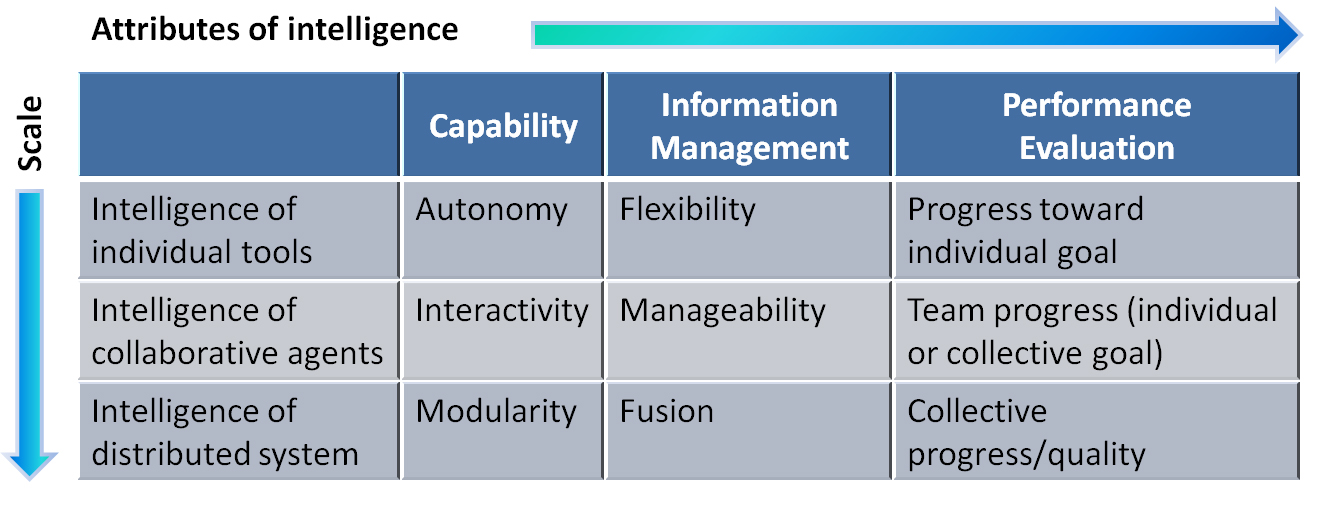
\includegraphics[width=3.5in]{IntegrationChallenges.JPG}
\caption{Autonomy integration challenges defined along two dimensions. Horizontal dimension: attributes of intelligence. Vertical dimension: scale.}
\label{IChallenges}
\end{figure}

Many approaches to autonomy management exist, such as \textit{Supervisory Control}, \textit{Mixed-initiative}, \textit{Collaborative Control}, \textit{Adjustable Autonomy}~\cite{Dorais1998AdjustableAutonomy,Dorais2001Designing} (also referred to as \textit{Sliding Autonomy}~\cite{Dias2008SlidingAutonomy} or \textit{Adaptive Automation}~\cite{Rouse1988Adaptive,Kaber2001Design}). The approach we propose falls under the category of \textbf{Adjustable Autonomy}. However with our approach the user can influence the behavior of the automous system along two new dimensions: a temporal dimension for how much time to allocate to the subtask, and a spatial dimension for where to set task constraints. These two dimensions are in addition to dimensions of \textit{Adjustable Autonomy} identified in the literature~\cite{Bradshaw2004Dimensions}. To evaluate the usefulness of the proposed autonomy management approach, we applied it to the task of UAV (Unmanned Aerial Vehicle) path planning to support Wilderness Search and Rescue (WiSAR).

UAVs used for WiSAR. 
Use probability distribution map and task-difficulty map.
Given fixed flying time, maximize probability of finding missing person.
In the temporal dimension, use use slider to choose time allocation for current path segment. Then join segments to form full path.
In the spatial dimension, add constraints. Constraints can be end points or no-fly zones (cite spencer's paper).





  and evaluate the usefulness of the approach against manual control and simple pattern path planning methods in a user study.



By managing autonomy along these two new dimensions, the user can 






 Results show that the sliding autonomy approach performs significantly better than the other two modes, and the performance of the human-automation team outperforms either human or automation working alone. And the users' mental workload, measured by a secondary task performance and NASA TLX, 









What if feedback
quick feedback
Human strategic, autonomy tactic




Ideally humans should be doing what humans are good at, and autonomy should be doing what autonomy is good at.


``Humans, though fallible, are functionally rich in reasoning strategies and their powers of observation, learning, and sensitivity to context.'' ~\cite{Bradshaw2013Seven}

David Woods and Eric Hollnagel summarized this phenomenon as the law of stretched systems: ''every system is stretched to operate at tits capacity; as soon as there is some improvement, for example in the form of new technology, it will be exploited to achieve a new intensity and tempo of activity.''  ~\cite{Woods2006Joint}





Although AI and robotics systems have grown to be able to handle increasingly complex tasks in uncertain environments, human assistance and supervision are often needed~\cite{Bainbridge1983Ironies}. 



Even for fully autonomous systems, human input can potentially improve the system's performance and safety. 




Human understands manual and pattern.
They don't really know how autonomy works.


In~\cite{Vicente1997Should} Vicente suggests to follow the ecological approach~\cite{Rasmussen1994Cognitive} and design interfaces compatible with the actual constraints of the environment so the operator's understanding corresponds to the actual behavior of the system. 

Our information management approach and proposed tools are compatible with these principles because they allow a user to infer causal relationship between user actions and autonomous behavior changes. The user interface designs enable the user to develop mental models of the system that match how the system truly works and thereby improve the human-automation interaction experience.




%=================================================================================
\section{Related Work}
\label{sec:RelatedWork6}

Drucker defines automation as a ``concept of the organization of work~\cite{Drucker2006Practice}.'' Goodrich and Schultz~\cite{Goodrich2007HRISurvey} define the HRI problem as ``understanding and shaping the interactions between one or more humans and one or more robots.'' They also specified robot-assisted search and rescue as a key area for HRI research.

In their 1978 seminal paper~\cite{Sheridan1978Human}, Sheridan and Verplank propose the idea of a \textit{Level of Autonomy} spectrum, with full teleoperation at one end and full autonomy at the other. In the middle, the robot could suggest actions to humans or make decisions before informing humans. Parasuraman et al.\ \cite{Parasuraman2000Model} extended this one-dimensional spectrum to four different broad functions: information acquisition, analysis, decision selection, and action implementation. In~\cite{Sheridan1992Telerobotics} Sheridan proposes \textit{Supervisory Control}, in which a human divides the task into a sequence of subtasks that the robot is capable of performing, and the human then provides guidance when the autonomous system cannot solve a problem on its own. In contrast to the top-down philosophy of supervisory control, a \textit{Mixed-initiative} approach advocates the idea of dynamically shifting tasks when necessary~\cite{Hearst1999Mixed}. \textit{Collaborative Control}, which can be thought of as an instance of mixed-initiative interaction, is a robot-centric model; instead of the human always being in-charge, the robot is treated as a peer and can make requests to humans through dialogs~\cite{Fong1999Collaborative}. \textit{Adjustable Autonomy}~\cite{Dorais2001Designing} (also referred to as \textit{Sliding Autonomy}~\cite{Dias2008SlidingAutonomy} or \textit{Adaptive Automation}~\cite{Rouse1988Adaptive}) is another type of mixed-initiative interaction, one that enables the human-automation team to dynamically and adaptively allocate functions and tasks among team members. Bradshaw et al.\ \cite{Bradshaw2004Dimensions} propose two dimensions of Adjustable Autonomy (descriptive and prescriptive) to address the two senses of autonomy (self-sufficiency and self-directedness) and discuss how permissions, obligations, possibilities, and capabilities can be adjusted. Bradshaw et al.\ \cite{Bradshaw2013Seven} also summarized some widespread misconceptions on autonomy and listed seven deadly myths of ``autonomous systems.''

Dorais et al.\ \cite{Dorais1998AdjustableAutonomy} discuss a framework for human-centered autonomous systems for a manned Mars mission. The system enables users to interact with these systems at an appropriate level of control but minimize the necessity for such interaction. Bradshaw et al.\ discuss principles and pitfalls of adjustable autonomy and human-centered teamwork, and then present study results on so-called ``work practice modeling'' and human-agent collaboration in space applications~\cite{Bradshaw2003AdjustableAutonomy}. In~\cite{Kaber2005Adaptive} Kaber et al.\ describe an experiment simulating an air traffic control task where manual control was compared to Adaptive Automation (AA). Results suggest that humans perform better with AA applied to sensory and psychomotor information-processing functions than with AA applied to cognitive functions; these results also suggest that AA is superior to completely manual control. Brookshire et al.\ present preliminary results for applying sliding autonomy to a team of robots performing coordinated assembling work to help the system recover from unexpected errors and to thereby increase system efficiency~\cite{Brookshire2004Preliminary}. Dias et al.\ identified six key capabilities that are essential for overcoming challenges in enabling sliding autonomy in peer-to-peer human-robot teams~\cite{Dias2008SlidingAutonomy}.

Human is an integral part of the human-automation team. When working with automation, the human often takes on the supervisor role. Bainbridge points out that automation requires the human operator to take additional management responsibilities~\cite{Bainbridge1983Ironies}, and Sartar identified in~\cite{Sarter1998Making} two automation management policies: \textit{management by consent} and \textit{management by exception}, defining whether the human always retain authority or can the system take initiative. For complex automations, the human tends to rely on his/her \textit{mental models} (defined by Norman in~\cite{Norman1983Some}) to manage the system. Moray~\cite{Moray1999Mental} provides a good summary of how mental models are used and proposes that mental models ``allow operators to think about causal structures and functions in systems which they must control....'' Goodrich and Boer present a case study of Adaptive Cruise Control design and explain how an automobile driver can switch among multiple mental models and use different management strategies~\cite{Goodrich2002Multiple, Goodrich2003Model}. Lee and See propose that because people respond to technology socially, trust guides reliance when unanticipated situations make it impractical or impossible to understand automation~\cite{Lee2004Trust}. Hoffman et al.\ \cite{Hoffman2013Trust} suggests ``active exploration for trusting''(AET) and hope this approach can promote both trust ``calibration'' and appropriate reliance. Moray also points out that the operator's internal model of the environmental and task dynamics can affect how the operator samples information from the environment, and display interfaces should be designed to attract the right amount of attention~\cite{Moray1990Designing}.

Properly evaluate human-robot interaction has always been a challenging problem due to the diversity of team setups, environmental contexts, and tasks involved. Many metrics have been proposed in the literature. Crandall and Goodrich proposed a metric called Neglect Time to measure interaction efficiency~\cite{Crandall2002Principles}. Together with Neglect Time, Olsen and Goodrich later added Task Effectiveness, Robot Attention Demand, Fan Out, and Interaction Effort to the list of Metrics~\cite{Olsen2003Metrics}. Steinfeld and et al.\ suggest some common metrics for standardizing task-oriented human-robot interaction~\cite{Steinfeld2006Common}. In~\cite{Olsen2007Evaluating}, Olsen presents a set of criteria for evaluating new UI systems. Crandall and Cummings propose in~\cite{Crandall2007Ddentifying} a set of metric classes that can predict how many robots should be in the team and the system effectiveness for single-operator controlling multiple robots. We follow guidelines provided in these papers to validate our proposed solution.

The goal of our research is to support fielded missions in the spirit of Murphy's work~\cite{Casper2003Human}. UAV technology has emerged as a promising tool in supporting WiSAR~\cite{Murphy2008Cooperative,Bourgault2003Coordinated}. In~\cite{Bourgault2006Optimal, Bourgault2004Coordinated} Bourgault et al.\ describe how to use a Bayesian model to create paths for a single UAV or multiple coordinated UAVs to maximize the amount of probability accumulated by the UAV sensors. In~\cite{Bourgault2008AugmentedNodes} they also include scalable collaborative human systems as augmented sensor nodes and created paths for human ground searchers.


Many path planning algorithms in the literature address obstacle avoidance while planning a path to reach a destination using A*~\cite{Quigley2005Towards}, LRTA*~\cite{Howlett2006Learning}, D*~\cite{Stentz1997Optimal}, Voroni diagrams~\cite{Bortoff2000Path,Beard2005Autonomous}, or probability roadmaps and rapidly-exploring random tree (RRTs)~\cite{Pettersson2006Probabilistic}. Hierarchical heuristics approaches were also developed, such as Hierarchical A* (HA*) by Holte et al.\ ~\cite{Holte1996Hierarchical}, hierarchical task-based real-time path planning by Naveed et al.\ ~\cite{Meuleau2007Hierarchical}, and Hierarchical-AO* (HiAO*) by Meuleau and Brafman~\cite{Naveed2010Hierarchical}. The algorithms we present solve a different path planning problem by generating paths that make efficient use of the limited travel time and maximizing the probability of finding the missing person. This is similar to the Vehicle Routing Problem~\cite{Laporte1992Vehicle} and the Orienteering Problem (OP)~\cite{Golden1987Orienteering}, which is a variation of the Traveling Salesman Problem (TSP) (with names such as Prize-Collecting TSP (PCTSP)~\cite{Gutin2002Traveling} or TSP with profits~\cite{Feillet2005Traveling}), and is known to be NP-Hard~\cite{Sokkappa1990Cost}. Vansteenwegen et al.\ \cite{Vansteenwegen2011Orienteering} gives a good survey on the topic of OP, and listed various approaches such as exact methods~\cite{Laporte1990Selective,Fischetti1998Solving,Ramesh1992Optimal}, approximation heuristic approaches~\cite{Mittenthal1992Insert,Chao1996Fast,Ramesh1992Optimal}, Genetic Algorithm approach~\cite{Tasgetiren2000Genetic}, and Ant Colony Optimization approach~\cite{Liang2006Ant}. These algorithms work well with OP problems of small number of nodes (21--100 nodes). However, our path planning problem requires up to 1800 nodes with added challenges of repeated visits and partial detection.
 
In order to intelligently plan paths for a UAV, it is necessary to understand missing person behaviors and generate a probability distribution of likely places to find the missing person. Many researchers analyzed past WiSAR cases in order to understand missing person behaviors~\cite{Setnicka1980Wilderness,Hill1998Lost,Syrotuck2000Analysis,Heth1998Characteristics,Koester2008Lost}.~\cite{Syrotuck2000Introduction} describes how to use mathematical models to calculate the probability of detection, probability of area and probability of success. He also describes an example search mission. Researchers also looked at systematically utilizing GIS (Geographic Information System) information for search and rescue applications~\cite{Ferguson2008GIS,Soylemez2006Utility}.

Due to factors such as lighting conditions, dense vegetation, or human observer cognitive workload, even when sensor footprint covers the location of the missing person, probability of detection can be less than 1. In the 1950's, Koopman discussed the uncertainties in the act of detecting hostile submarines with radars and proposed a concept called the instantaneous probability of detection by one glimpse~\cite{Koopman1956Theory}. He presented simple search algorithms and demonstrated how search effort should be distributed given a prior probability distribution of the target and known law of detection when only a limited total amount of search effort (or time) is available~\cite{Koopman1957Theory}. Stone~\cite{Stone1975Theory} presents various search plans with partial detection models using Lagrange multipliers and maximization of Lagrangians in finding stationary target in very basic search problems when no false targets are present. Washburn~\cite{Washburn1981Search} discusses how to construct optimal search paths for different search problems. The author also developed detection models based on radar/sonar and expanded the fundamentals of search theory to include moving targets. More recent work includes~\cite{Niedfeldt2010integrated} where Niedfeldt et al.\ present a UAV path planning algorithm that utilizes probability of detection and maximizes the probability of identifying an object using a N-step lookahead method, and~\cite{Ryan2010particle} where Ryan and Hedrick developed a control formulation for a fixed-wing UAV that minimizes the entropy of an estimate distribution over a receding horizon for searching a moving target over a fixed time horizon. Stone et al.\ used posterior probability maps and successfully located the wreckage of Air France Flight 447~\cite{Stone2011Search}. Metrics such as Koopman's instantaneous probability of detection by one glimpse~\cite{Koopman1956Theory}, ``seeability'' proposed by Morse et al.\ \cite{Morse2010UAV}, and terrain and vegetation information obtained from USGS~\cite{Lin2010Bayesian} can be used to build a task-difficulty map representing probability of detection in different search subregions.

The UAV technology is an intelligent system with the integration of many component autonomous algorithms and user interfaces. Integration at this level requires tremendous effort. Salas and Fiore~\shortcite{Salas2004Team} provide great insights on challenges across people and machines, and across time and space in distributed teams. Sycara and Lewis~\shortcite{Sycara2002Integrating} also asked the questions: 1) can a software agent perform the task? and 2) can the agent's assistance contribute toward team performance? Tso et al.\ ~\shortcite{Tso1999Multi} identified that integrating a UAV into the search task creates at least two roles: a pilot that controls the UAV and a sensor operator that analyzes the sensor outputs, and lessons from other search-related domains~\cite{Drury2003Awareness} show that multiple roles are required and these roles can be supported by autonomy algorithms and user interface technologies. These findings motivate and guide our research in developing UAV technology to support WiSAR operations.



%=================================================================================	
\section{Hypotheses} 
\label{sec:Hypotheses}


The BYU WiSAR research group has developed a variety of technologies to support Wilderness Search and Rescue with small fixed-wing UAVs~\cite{Beard2005Autonomous, Goodrich2008Supporting, Goodrich2009Towards, Lin2010Supporting}. The UAV system has many autonomous capabilities. The UAV's autopilot can stabilize the UAV during flight, support waypoint following and auto launch/land modes, and provide gimbaled camera control. Simple flight patterns and safety features are available when combining the autopilot with UAV control interfaces~\cite{Beard2005Autonomous, Lin2010Supporting}. These basic UAV capabilities have been greatly extended to provide better WiSAR support: A Bayesian model was developed by Lin and Goodrich~\cite{Lin2010Bayesian} that uses terrain features to predict the likely locations of finding a lost person. Then, Generalized Contour Search~\cite{Goodrich2008Supporting} and Intelligent Path Planning~\cite{Lin2009UAV,Niedfeldt2010integrated} algorithms have been used to automatically generate flight paths for the UAV. A real-time temporally local mosaic technique~\cite{Morse2008Application} has been used to ``stitch'' multiple video frames to provide increased opportunity for detection and increased sense of relative spatial relationships for video analyst. Anomaly detection algorithms~\cite{Thornton2011Unusual} are also available that can mark objects with unnatural colors and alert the video analyst. A metric named ``see-ability''~\cite{Morse2010UAV} was also developed to understand search-related video quality and to index geo-tagged video frames. 


%=================================================================================	
\section{User Study Design} 
\label{sec:Design}

%===================================================
\subsection{Participants}

%===================================================
\subsection{Simulation Environement}

%===================================================
\subsection{Scenarios}

%===================================================
\subsection{Procedure}

%===================================================
\subsection{Measures}



%=================================================================================	
\section{Results} 
\label{sec:Results}




%=================================================================================	
\section{Discussion} 
\label{sec:Discussion}




%=================================================================================	
\section{Conclusions and Future Work} 
\label{sec:Conclusions6}


The \textbf{SlidingAutonomy} interface allows the user to work with automation as a team and affect the behavior of the path planning autonomy by setting constraints and play with different flight duration. The user study we performed is a short-term study where each user only had a short training before using this interface. Because human's trust in autonomy can change over time, it would be interesting to research how the user's trust gets calibrated when the user uses this autonomy management approach for a long period of time. Would the user be able to gradually identify the weaknesses of the path planning autonomy and remedy correctly? Would the user overtrust autonomy and perform worse in the long run? Or would the user undertrust autonomy because autonomy makes obvious mistakes in certain scenarios? In our user study, the two scenarios used are both relatively easy scenarios. When more complicated \textit{probability distribution map} and \textit{task-difficulty map} are used, the benefit of using the \textbf{Sliding Autonomy} interface might be more obvious, and it would interesting to investigate how users would react to that. It is also possible to let the user specify the number of top regions through the \textbf{Sliding Autonomy} interface for the Top2 and TopN algorithms and see how that would affect the human-automation interaction. These questions can only be answered with a long-term user study, which we leave for future work.

At this scale, while the UAV is in the air during mission, as information is collected and processed by the collective search and rescue team, situation arises when the \textit{probability distribution map} and/or the \textit{task-difficulty map} become incorrect. In cases where these two maps cannot be updated in real-time, how can the user use \textbf{SlidingAutonomy} to manage UAV path planning autonomy to address the information change, maybe avoid certain regions or force the UAV to visit certain regions repeatedly, is another interesting research topic. A user study can be performed to evaluate the human-automation interaction experience and the performance of this Sliding Autonomy approach.



%=================================================================================	
\section*{Acknowledgments}

This work was partially supported by 
the National Science Foundation 
%\_\_\_\_\
under grant number 
0534736 
%\_\_\_\_\_
and by a grant from
the Army Research Laboratory.
%\_\_\_\_\.
Any opinions, findings, and conclusions or recommendations expressed in this material are those of the authors and do not necessarily reflect the views of the sponsoring organizations.

%% Use plainnat to work nicely with natbib. 

\bibliographystyle{IEEEtran}
\bibliography{LannyDissertation}


\end{document}